\documentclass{article}
\usepackage[T1]{fontenc}
\usepackage{lmodern}
\usepackage{graphicx}
\usepackage{amsmath,amssymb}
\usepackage[a4paper,margin=2cm]{geometry}
\usepackage[absolute,overlay]{textpos}
\setlength{\TPHorizModule}{1mm}
\setlength{\TPVertModule}{1mm}
\usepackage[indonesian]{babel}
\usepackage{hyperref}
\setlength{\emergencystretch}{2em}
% unit: Halaman 9

\begin{document}

% === Halaman 9 (llm) ===

\begin{itemize}
    \item \textbf{Case 4:} Bagaimana Bob melakukan anti-sangkalan apabila Alice menyangkal telah mengirim pesan kepada Bob?
\end{itemize}

\textcolor{red}{Swer, saya nggak pernah kirim pesan ini kepadamu, Bob!} \hfill \textcolor{red}{Hmmmmm....}

\vspace{30mm}

$\rightarrow$ masalah nir-penyangkalan (non-repudiation)

% deskripsi: Diagram ilustrasi pengiriman pesan dari Alice ke Bob yang menggambarkan masalah non-repudiation, dengan panah menunjukkan aliran pesan dan karakter Alice dan Bob.
% bbox normalisasi: [0.1800, 0.4500, 0.7600, 0.7100]
\begin{textblock*}{121.80mm}(37.80mm,133.65mm)
\noindent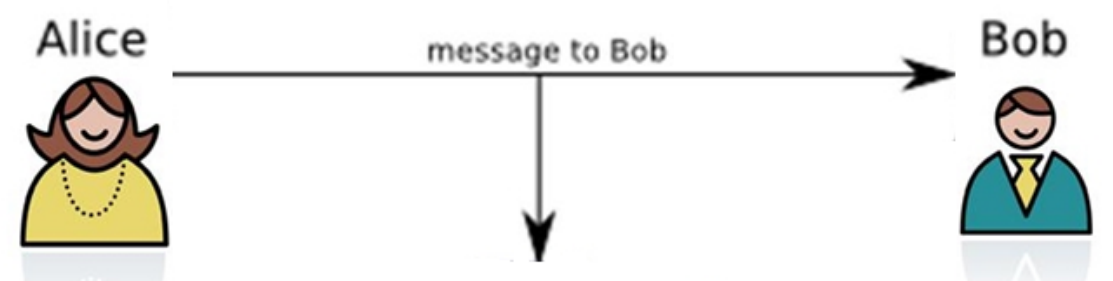
\includegraphics[width=121.80mm,height=77.22mm]{../../images/llm/page_009_img_01.png}%
\end{textblock*}

\end{document}
